%--------------------------------------------%
% Template Beamer para Apresentações da UFRN %
% by alcemygvseverino@gmail.com              %
% Baseado em MIT Beamer Template			 %
% versao 1.1								 %
% Atualizado em 14/05/2016					 %
%--------------------------------------------%
\documentclass[]{beamer}

\mode<presentation>
{
% Para definir o tema do slide
\usetheme{Berlin}
% Para difinir cores e background
\usecolortheme{ufrn}
% Para numerar as figuras
\setbeamertemplate{caption}[numbered]
	\setbeamercovered{transparent}
}

% Para alterar a linguagem do documento
\usepackage[spanish]{babel}
% Para aceitar caracteres especias deretamente do teclado
\usepackage[utf8]{inputenc}
% Para seguir as normas da ABNT de citacao e referencias
\usepackage[alf]{abntex2cite}
% Para incluir figuras
\usepackage{graphicx}
% Para melhor ajuste da posisao das figuras
\usepackage{float}
% Para ajustar as dimensoes do layout da pagina
\usepackage{geometry}
% Para formatar estrutura e informacoes de formulas matematicas
\usepackage{amsmath}
% Para incluir simbolos especiais em formulas matematicas
\usepackage{amssymb}
% Para incluir links nas referencias
\usepackage{url}
% Para incluir paginas de documentos .pdf externos
\usepackage{pgfpages}
% Para ajustar o estilo dos contadores
\usepackage{enumerate}
% Para modificar a cor do texto
\usepackage{color}
% Para incluir condicoes
\usepackage{ifthen}
% Para colocar legendas em algo que nao e float
\usepackage{capt-of}
\usepackage{hyperref}
\usepackage{algorithm,algorithmic}
\usepackage{colortbl}

%\usepackage[T1]{fontenc}
\usepackage{inconsolata}
\usepackage{listings}

\lstset{language=Java,
basicstyle=\footnotesize\tt,        % the size of the fonts that are used for the code
 breakatwhitespace=false,         % sets if automatic breaks should only happen at whitespace
 breaklines=true,                 % sets automatic line breaking
 captionpos=b,                    % sets the caption-position to bottom
 extendedchars=true,              % lets you use non-ASCII characters; for 8-bits encodings only, does not work with UTF-8
 frame=single,                    % adds a frame around the code
 language=Java,                 % the language of the code
 keywordstyle=\bf,
 showspaces=false,                % show spaces everywhere adding particular underscores; it overrides 'showstringspaces'
 showstringspaces=false,          % underline spaces within strings only
 showtabs=false,                  % show tabs within strings adding particular underscores
 tabsize=2                       % sets default tabsize to 2 spaces
}


% Título

\title[Programaci\'on 2]{Programaci\'on 2}
\subtitle{Lenguaje Java - Patrones de Diseño )\\ T\'ipos de Clases}
% Data
\date{
	\today}
% Autores
\author[Eduardo Godoy]{
	Profesor: Eduardo Godoy. \\
	\vspace{0.5mm}
	\texttt{\small eduardo.gl@gmail.com}
}
}
\institute[Universidad de Valara\'iso]{
	\vspace{0.25cm}
	\texttt Escuela de Ingenier\'ia Civil Inform\'atica.\\
	\texttt Universidad de Valpara\'iso.
}

\begin{document}

\frame{\titlepage}
\section[]{}
\begin{frame}{Contenido}
	\tableofcontents
\end{frame}
\section{Introduci\'on.}

\begin{frame}{Introducci\'on.}
	\begin{itemize}
		\item Se sabe que cada Aplicaci\'on tiene particularidades.
		\item Pero en general  siempre se repiten los mismos problemas:
			\begin{block}{Problemas recurrentes al desarrollar una aplicaci\'on}
			\begin{itemize}
				\item ?`C\'omo persisto los datos?
				\item ?`C\'omo autentifico a los usuarios?
				\item ?`C\'omo separo la presentaci\'on, la l\'ogica y control?.
			\end{itemize}
		\end{block}
					\item En lugar de reinventar continuamente una soluci\'on para cada nuevo proyecto. Es mucho mas
					productivo aplicar estrategias que ya hayan funcionado anteriormente.
					\item Esta idea es lo que lleva al concepto de \textit{ \textbf{Patr\'on de Diseño} }.
	\end{itemize}
\end{frame}

\begin{frame}{Patr\'on -> Un Modelo}
	\begin{itemize}
		\item En ingenier\'ia del software, un	patr\'on es una soluci\'on ya probada y aplicable a un
		problema que se presenta una y otra vez en el desarrollo de distintas aplicaciones y en
		distintos contextos.
		\item Un patr\'on no es una soluci\'on  codificada y lista para usar, sino más bien un \textbf{modelo}
		que describe c\'omo resolver el problema y de ante qu\'e circunstancias es aplicable.
		\item Si se decide aplicar un patr\'on, este debe ser previamente comunicado y documentado con el equipo del proyecto.
	\end{itemize}
\end{frame}

\begin{frame}{Patr\'on - Ventajas}
	\begin{itemize}
		\item \textbf{Están Probados:} son soluciones que han sido utilizadas con anterioridad de manera
		repetida y se ha comprobado que funcionan.
		\item \textbf{Son reutilizables:} corresponden con problemas que no son espec\'ificos de un caso
		concreto, sino que se presentan de forma recurrente en distintas aplicaciones.
		\item \textbf{Son expresivos:} cuando un equipo de desarrolladores tiene un vocabulario com\'un de
		patrones, se puede comunicar de manera fluida y precisa las ideas fundamentales sobre
		el dise\~no de una aplicaci\'on.
	\end{itemize}
\end{frame}

\begin{frame}{Patr\'on - Desventajas}
	\begin{itemize}
		\item Uso sin justificaci\'on que no aplica a un problema. (Simplemente porque son buenos)
		\item El an\'alisis y experiencia debe dictar si es necesario o no aplicarlos.
	\end{itemize}
\end{frame}


%\begin{frame}{Tips - Ocultamiento de Informaci\'on - Ejemplo.}
  %\begin{figure}
    %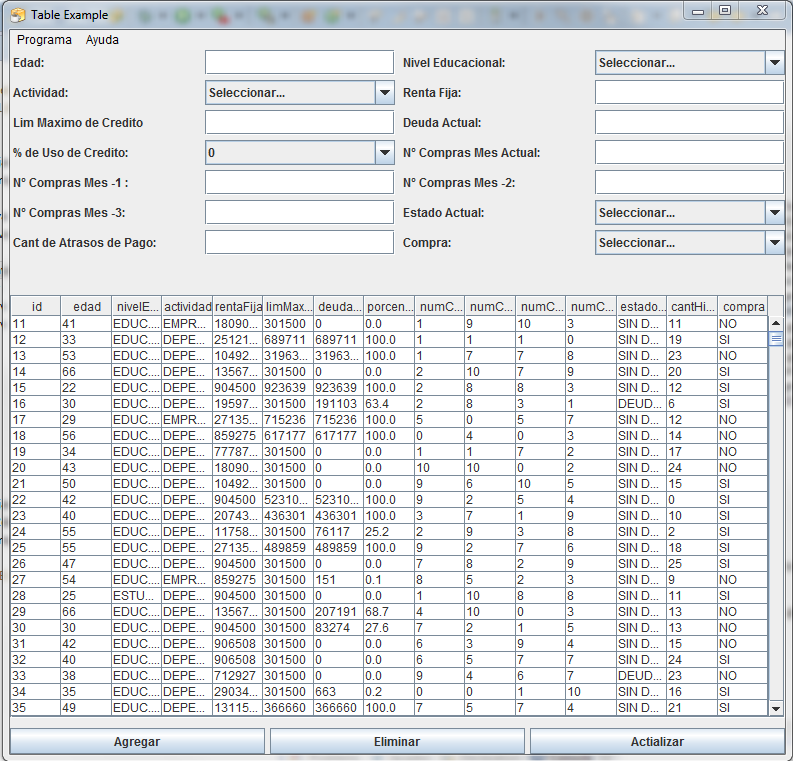
\includegraphics[scale=0.3]{figuras/DT.PNG}
  %\end{figure}
%\end{frame}

%\begin{frame}{Manejo de Excepciones - try, catch, finally}
%\begin{block}{Ejemplo.}
%\lstinputlisting[language=Java,caption={},numbers=none]{resources/excepciones/Finally.java}
%\end{block}
%\end{frame}

\section{DAO - \emph{Data Acceso Object}}

\begin{frame}{DAO - \emph{Data Acceso Object}}
	\begin{itemize}
		\item DAO Es un patrón de diseño del tipo creacional.
		\item Est\'a basado directamente en el concepto de \emph{Separaci\'on de Responsabilidades}.
		\begin{block}{Separaci\'on de Responsabilidades.}
		\begin{itemize}
			\item Cada clase es creada bajo un \'unico fin o responsabilidad asignada.
			\item La responsabilidad debe ser cumplida en su totalidad por la clase.
			\item Este concepto define que una responsabilidad debe estar asociado de forma directa a solo un clase.
		\end{itemize}
		\end{block}
	\end{itemize}

\end{frame}

\begin{frame}{DAO - Responsabilidad}
	\begin{itemize}
		\item En una aplicación empresarial, DAO tiene la responsabilidad de separar la persistencia de datos del resto de funcionalidades.
		\item Esto proporciona \emph{independencia de la fuente de datos}, al tener dicha responsabilidad encapsulada dentro de la misma clase.
		\begin{block}{Nota Relevante}
		\begin{itemize}
			\item Un principio b\'asico de un buen diseño de sistema es identificarlos aspectos de la aplicacion
						que cambian o pueden cambiar y separarlos de los que van a permanecer siempre fijos. Muchos patrones de diseño se basan en encapsular de alguna forma
						la parte que cambia para hacer mas f\'acil la extensi\'on del sistema.
			\item DAO encapsula la parte que puede cambiar, que es la interacci\'on con la fuente de datos.
		\end{itemize}
		\end{block}
	\end{itemize}

\end{frame}

%\begin{frame}{Tips - Ocultamiento de Informaci\'on - Ejemplo.}
  %\begin{figure}
    %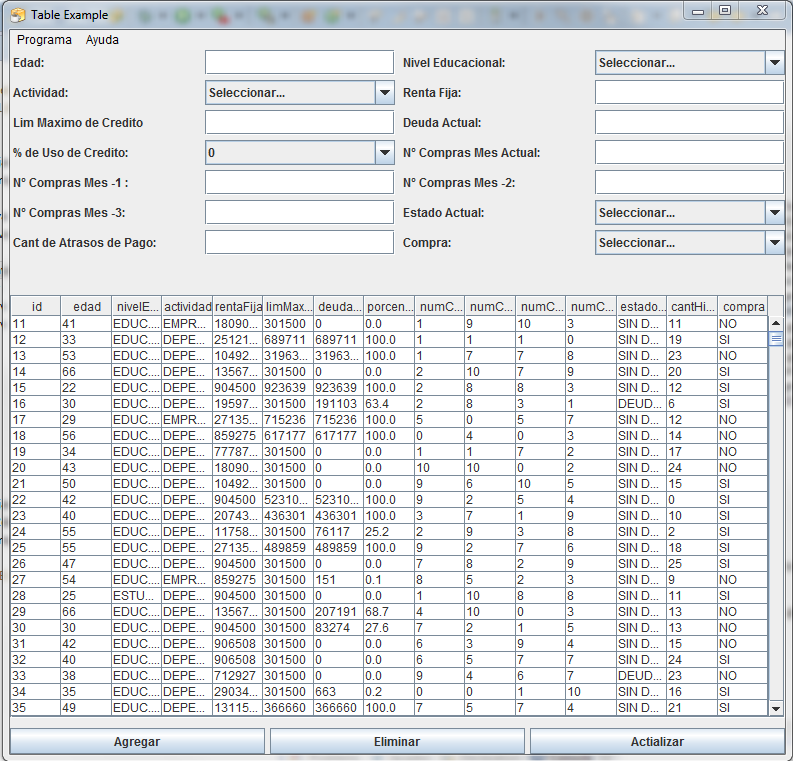
\includegraphics[scale=0.3]{figuras/DT.PNG}
  %\end{figure}
%\end{frame}

%\begin{frame}{Manejo de Excepciones - try, catch, finally}
%\begin{block}{Ejemplo.}
%\lstinputlisting[language=Java,caption={},numbers=none]{resources/excepciones/Finally.java}
%\end{block}
%\end{frame}

\section{MVC - \emph{Model View Controller.}}
\begin{frame}{Introducci\'on}
\begin{block}{}
	\begin{itemize}
		\item Patr\'on de diseño que separa al modelo de datos, la lógica de control de la aplicaci\'on y la interfaz de usuario en tres componentes distintos.
		\item Propone la implementaci\'on de 3 componentes caracterizados por:
			\begin{itemize}
				\item Tener muchas interfaces de usuario.
				\item Tener muchos controladores.
				\item Tener un solo modelo.
			\end{itemize}
	\end{itemize}
\end{block}
\end{frame}

\begin{frame}{Componentes}
	\begin{itemize}
		\item Modelo: Representaci\'on del modelo de dominio,  logica del negocio
		\item View: Interfaz de usuario e interacci\'on entre elementos de la interfaz.
		\item The controller: Intermediario entre modelo y vista, recibe los evntos ejecutados por el usuario y solicita al modelo los datos requeridos producto del evento.
		\end{itemize}
\end{frame}

\begin{frame}{Esquema - MVC.}
  \begin{figure}
    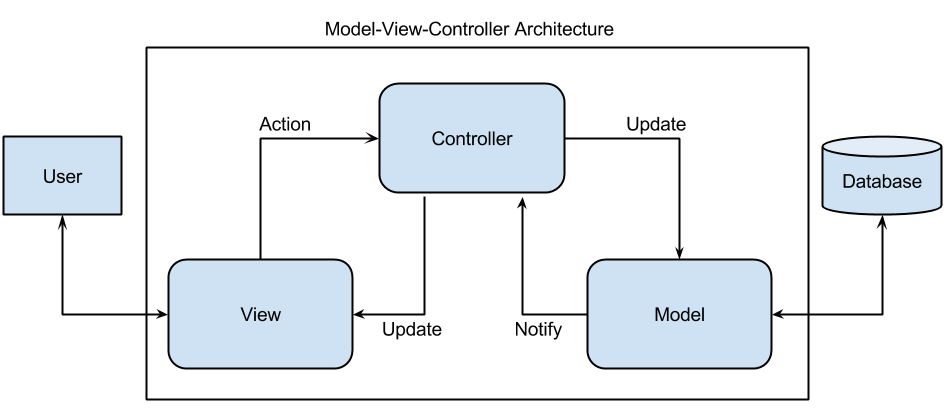
\includegraphics[scale=0.3]{figuras/Model-View-Controller-High-Level-Diagram.png}
  \end{figure}
\end{frame}

\begin{frame}{Beneficios}
	\begin{itemize}
		\item Organizaci\'on.
		\item Desarrollo de aplicaci\'on r'apido.
		\item Reutilizaci\'on de c\'ondigo.
		\item Desarrollo de software paralelo.
		\item Permite representar la misma informaci\'on de distintas maneras.

	\end{itemize}
\end{frame}




%\begin{frame}{Tips - Ocultamiento de Informaci\'on - Ejemplo.}
  %\begin{figure}
    %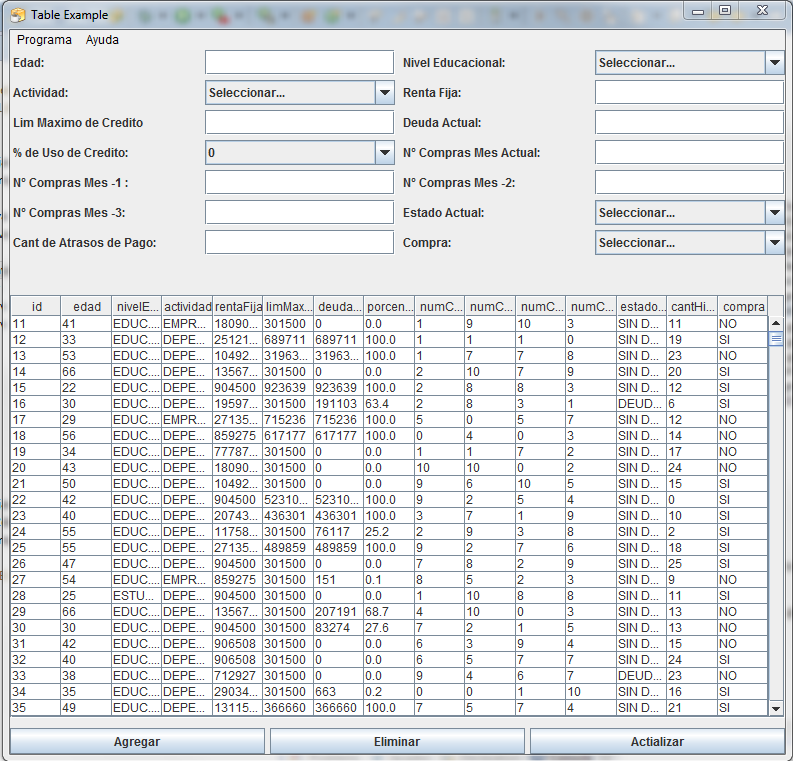
\includegraphics[scale=0.3]{figuras/DT.PNG}
  %\end{figure}
%\end{frame}

%\begin{frame}{Manejo de Excepciones - try, catch, finally}
%\begin{block}{Ejemplo.}
%\lstinputlisting[language=Java,caption={},numbers=none]{resources/excepciones/Finally.java}
%\end{block}
%\end{frame}

\section{}
%\begin{frame}{Agradecimentos}
%	Agradeço a todos.
%\end{frame}

\end{document}
